\documentclass[10pt,pdf,hyperref={unicode}]{beamer}

\mode<presentation>
{
\usetheme{boxes}
\beamertemplatenavigationsymbolsempty

\setbeamertemplate{footline}[page number]
\usecolortheme{seagull}
\setbeamersize{text margin left=0.5em, text margin right=0.5em}
}

\usepackage[utf8]{inputenc}
\usepackage[english, russian]{babel}
\usepackage{bm}
\usepackage{multirow}
\usepackage{ragged2e}
\usepackage{indentfirst}

\newtheorem{rustheorem}{Теорема}

\AtBeginEnvironment{figure}{\setcounter{subfigure}{0}}% Resets subfigure counter at start of figure environment

%----------------------------------------------------------------------------------------------------------
\title[\hbox to 56mm{истилляция и привилегированная информация \hfill\insertframenumber\,/\,\inserttotalframenumber}]
{Привилегированная информация и дистиляция моделей}
\author[А.\,В.~Грабовой]{\large \\Грабовой Андрей Валериевич}
\institute{\large
Московский физико-технический институт}

\date{\footnotesize{МФТИ, г. Долгопрудный}}
%----------------------------------------------------------------------------------------------------------

\begin{document}
%----------------------------------------------------------------------------------------------------------
\begin{frame}
\titlepage
\end{frame}

%----------------------------------------------------------------------------------------------------------
\begin{frame}{Вероятностная интерпретация дистилляции моделей}
\justifying
\textbf{Цель:} предложить вероятностную постановку задачи дистилляции моделей глубокого обучения на основе существующих методов дистилляции и привилегированного обучения.
%предложить метод построения ансамбля локально аппроксимирующих моделей для поиска окружностей на изображении.



~\\
\textbf{Задачи}

\begin{enumerate}
\justifying
	\item Поставить вероятностную задачу дистилляции для задачи классификации и регрессии.
	%Предложить метод поиска окружности при помощи линейной модели, для поиска нескольких окружностей предложить метод построения смеси локальных аппроксимирующих моделей.
	\item Провести теоретический анализ предложенной вероятностной постановки задачи для линейных моделей.
	%Предложить априорные распределения на параметры локальных моделей.
\end{enumerate}

~\\
\textbf{Исследуемая проблема:} снижение размерности пространства параметров моделей глубокого обучения.

~\\
\textbf{Метод решения}

	Предлагается поставить вероятностную постановку задачи дистилляции моделей глубокого обучения. В качестве базовой дистилляции предлагается использовать методы предложенные Дж. Хинтоном и В. Вапником в 2015г. и 2016г. соответсвенно.
	
\end{frame}

%----------------------------------------------------------------------------------------------------------
\begin{frame}{Список литературы}
\justifying
\begin{enumerate}
	\item \textit{Грабовой А.В., Стрижов В.В.} Анализ моделей привилегированного обучения и дистилляции // Автоматика и телемеханика, 2021 (текущая работа, на рецензировании).
	\item \textit{Lopez-Paz D., Bottou L., Scholkopf B., Vapnik V.} Unifying Distillation and Privileged Information // In International Conference on Learning Representations. Puerto Rico, 2016.
	\item \textit{Hinton G., Vinyals O., Dean J.} Distilling the Knowledge in a Neural Network // NIPS Deep Learning and Representation Learning Workshop. 2015.
	\item \textit{Madala H., Ivakhnenko A.} Inductive Learning Algorithms for Complex Systems Modeling. Boca Raton: CRC Press Inc., 1994.
\end{enumerate}
\end{frame}

%----------------------------------------------------------------------------------------------------------

\begin{frame}{Введения}
\justifying
\begin{center}
	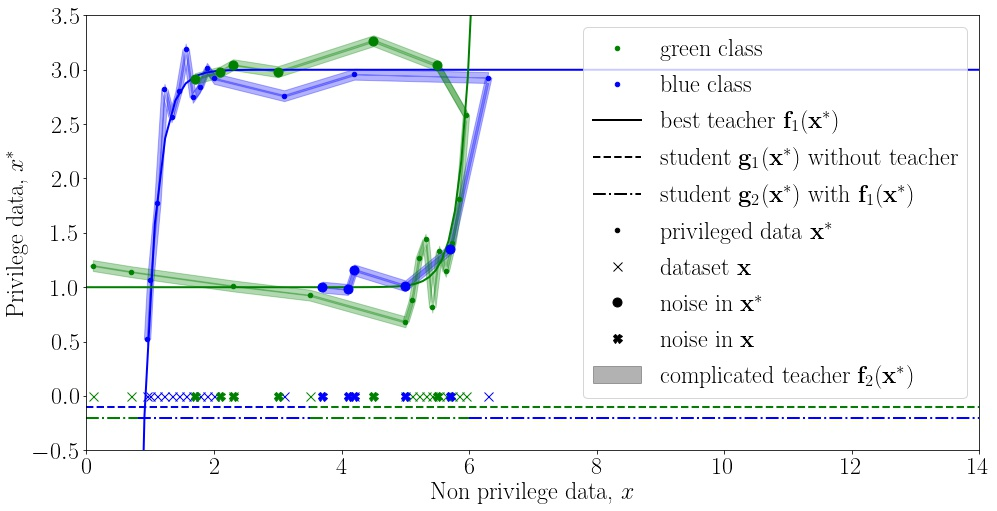
\includegraphics[width=0.8\textwidth]{figures/explanation}
\end{center}
\end{frame}
%----------------------------------------------------------------------------------------------------------
\begin{frame}{Постановка задачи обучения с учителем}
\justifying
Множество объектов~$\bm{\Omega},$ где $\left|\bm{\Omega}\right| = m$.

Признаки~$\mathbf{x}_i = \varphi(\omega_i),$ где $\mathbf{x}_i \in \mathbb{R}^{n}$.
Целевая переменная~$y_i = y\bigr(\omega_i\bigr),$ $y_i \in \mathbb{Y}$.

Привилегированные признаки~$\varphi^*(\omega_i)=\mathbf{x}^*_i \in \mathbb{R}^{n^*},$ где  $\omega_i\in \bm{\Omega}' \subseteq \bm{\Omega}$.

Множество индексов объектов, для которых известна привилигированя информация обозначим $\mathcal{I},$ а $\bar{\mathcal{I}}$ для которых не известная.

Функции учителя~$\mathbf{f}:\mathbb{R}^{n^*} \to \mathbb{Y}^*$ и ученика~$\mathbf{g}:\mathbb{R}^{n} \to \mathbb{Y}^*,$ где~$\mathbb{Y}^*$ пространство оценок.

Ответ функции $\mathbf{f}$ для объекта~$\mathbf{x}^*_i$ обозначим~$\mathbf{s}_i = \mathbf{f}\bigr(\mathbf{x}_i^*\bigr)$.

Требуется выбрать модель ученика~$\mathbf{g}$ из множества:
\[
\setlength\abovedisplayskip{0pt}
	\mathfrak{G} = \left\{\mathbf{g}| \mathbf{g}:\mathbb{R}^{n} \to \mathbb{Y}^*\right\}.
\setlength\belowdisplayskip{0pt}
\]

Например: 
\[
\setlength\abovedisplayskip{0pt}
	\mathfrak{G}_\text{lin,cl} = \left\{\mathbf{g}\bigr(\mathbf{W}, \mathbf{x}\bigr)| \mathbf{g}\bigr(\mathbf{W}, \mathbf{x}\bigr) = \text{softmax}\bigr(\mathbf{W}\mathbf{x}\bigr), \quad \mathbf{W} \in \mathbb{R}^{n\times K}\right\},
\setlength\belowdisplayskip{0pt}
\]
где $\mathfrak{G}_\text{lin,cl}$ параметрическое семейство линейный моделей для задачи классификации.

Оптимизационная задача:
\[
\setlength\abovedisplayskip{0pt}
	\mathbf{g} = \arg\min_{\mathbf{g} \in \mathfrak{G}} \mathcal{L}\bigr(\mathbf{g}, \mathbf{f}, \mathbf{X}, \mathbf{X}^{*}, \mathbf{y}\bigr),
\setlength\belowdisplayskip{0pt}
\]
где $\mathcal{L}$ некоторая функция ошибки.
\end{frame}
%----------------------------------------------------------------------------------------------------------
\begin{frame}{Постановка задачи: Хинтон}
\justifying
Рассматривается:
\begin{enumerate}
	\item $\mathcal{I} = \{1, 2, \cdots, m\}$;
	\item для всех $i \in \mathcal{I}$ выполняется $\mathbf{x}_i = \mathbf{x}^*_i$;
	\item классификация $\mathfrak{D} = \{\left(\mathbf{x}_i, y_i\right)\}_{i=1}^{m}, \mathbf{x}_i \in \mathbb{R}^{n}, y_i \in \mathbb{Y}=\{1, \cdots, K\}$.
\end{enumerate}
Обозначим~$y_i$~--- класс объекта, а~$\mathbf{y}_i$ вектор вероятности для~$i$-го объекта.

Параметрическое семейство учителя и ученика:
\[
\setlength\abovedisplayskip{0pt}
\mathfrak{F}_{\text{cl}} = \left\{\mathbf{f}| \mathbf{f} = \text{softmax}\bigr(\mathbf{v}\bigr(\mathbf{x}\bigr)/T\bigr), \quad \mathbf{v}: \mathbb{R}^n \to \mathbb{R}^K \right\},
\setlength\belowdisplayskip{0pt}
\]
\[
\setlength\abovedisplayskip{0pt}
\mathfrak{G}_{\text{cl}} = \left\{\mathbf{g}| \mathbf{g} = \text{softmax}\bigr(\mathbf{z}\bigr(\mathbf{x}\bigr)/T\bigr), \quad \mathbf{z}: \mathbb{R}^n \to \mathbb{R}^K \right\},
\setlength\belowdisplayskip{0pt}
\]
где~$\mathbf{z},\mathbf{v}$~--- это дифференцируемые параметрические функции заданной структуры, $T$~--- параметр температуры.

Функция потерь~$\mathcal{L}_{st}$:
\[
\setlength\abovedisplayskip{0pt}
\begin{aligned}
   \mathcal{L}_{st}\bigr(\mathbf{g}\bigr) = &-\sum_{i=1}^{m}\underbrace{{\sum_{k=1}^{K}y^k_i\log\mathbf{g}\bigr(\mathbf{x}_i\bigr)\bigr|_{T=1}}}_{\text{исходная функция потерь}}- \sum_{i=1}^{m}\underbrace{{\sum_{k=1}^{K}\mathbf{f}\bigr(\mathbf{x}_i\bigr)\bigr|_{T=T_0}\log\mathbf{g}\bigr(\mathbf{x}_i\bigr)\bigr|_{T=T_0}}}_{\text{слагаемое дистилляция}},
\end{aligned}
\setlength\belowdisplayskip{0pt}
\]
где~$\cdot\bigr|_{T=t}$ обозначает, что параметр температуры~$T$ в предыдущей функции равняется~$t$.

Получаем оптимизационную задачу:
\[
\setlength\abovedisplayskip{0pt}
	\hat{\mathbf{g}} = \arg\min_{\mathbf{g} \in \mathfrak{G}_{\text{cl}}} \mathcal{L}_{st}\bigr(\mathbf{g}\bigr).\setlength\belowdisplayskip{0pt}
\]

\end{frame}
%----------------------------------------------------------------------------------------------------------
\begin{frame}{Постановка задачи: Вапник}
\justifying
Рассматривается:
\begin{enumerate}
	\item привилегированная информация~$\mathcal{I} = \{1, 2, \cdots, m\}$;
	\item классификация $\mathcal{D} = \left\{\left(\mathbf{x}_i, \mathbf{x}^*_i, y_i\right)\right\}_{i=1}^{m}, \mathbf{x}_i \in \mathbb{R}^{n}, \mathbf{x}^*_i \in \mathbb{R}^{n^*}, y_i \in \{1, \cdots, K\}$.
\end{enumerate}
Параметрическое семейство учителя:
\[
\setlength\abovedisplayskip{0pt}
\mathfrak{F}_{\text{cl}}^* = \left\{\mathbf{f}| \mathbf{f} = \text{softmax}\bigr(\mathbf{v}^*\bigr(\mathbf{x}^*\bigr)/T\bigr), \quad \mathbf{v}^*: \mathbb{R}^{n^*} \to \mathbb{R}^K \right\},
\setlength\belowdisplayskip{0pt}
\]
где~$\mathbf{v}^*$~--- это дифференцируемые параметрические функции заданной структуры, $T$~--- параметр температуры.

Функция потерь:
\[
\setlength\abovedisplayskip{0pt}
\begin{aligned}
   \mathcal{L}_{st}\bigr(\mathbf{g}\bigr) = &-\sum_{i=1}^{m}{\sum_{k=1}^{K}y^k_i\log\mathbf{g}\bigr(\mathbf{x}_i\bigr)\bigr|_{T=1}}-\sum_{i=1}^{m}{\sum_{k=1}^{K}\mathbf{f}\bigr(\mathbf{x}^*_i\bigr)\bigr|_{T=T_0}\log\mathbf{g}\bigr(\mathbf{x}_i\bigr)\bigr|_{T=T_0}},
\end{aligned}
\setlength\belowdisplayskip{0pt}
\]
где~$\cdot\bigr|_{T=t}$ обозначает, что параметр температуры~$T$ в предыдущей функции равняется~$t$.

\end{frame}
%----------------------------------------------------------------------------------------------------------
\begin{frame}{Вероятностная постановка}
\justifying
Гипотеза порождения данных:
\begin{enumerate}
	\item задано распределение целевой переменной~$p\bigr(y_i|\mathbf{x}_i, \mathbf{g}\bigr)$;
	\item задано совместное распределение~$p\bigr(y_i, \mathbf{s}_i|\mathbf{x}_i, \mathbf{g}\bigr)$;
	\item для всех $i \in \mathcal{I}$ элементы $y_i$ и $\mathbf{s}_i$ являются зависимыми величинами;
	\item если $|\mathcal{I}|=0$ то решение cоответствует решению максимума правдоподобия.
\end{enumerate}
Совместное правдоподобие истинных меток и меток учителя:
\[
\setlength\abovedisplayskip{0pt}
p\bigr(\mathbf{y}, \mathbf{S}|\mathbf{X}, \mathbf{g}, \mathcal{I}\bigr)=\prod_{i\not\in \mathcal{I}}p\bigr(y_i|\mathbf{x}_i, \mathbf{g}\bigr)\prod_{i\in \mathcal{I}}p\bigr(y_i, \mathbf{s}_i|\mathbf{x}_i, \mathbf{g}\bigr).
\setlength\belowdisplayskip{0pt}
\]
Задача оптимизации:
\[
\setlength\abovedisplayskip{0pt}
\mathbf{g} = \arg\max_{\mathbf{g} \in \mathfrak{G}} p\bigr(\mathbf{y}, \mathbf{S}|\mathbf{X}, \mathbf{g}, \mathcal{I}\bigr),
\setlength\belowdisplayskip{0pt}
\]
данная задача оптимизации переписывается в следующем виде:
\[
\setlength\abovedisplayskip{0pt}
\begin{aligned}
\hat{\mathbf{g}} = \arg\max_{\mathbf{g}\in \mathcal{G}} \sum_{i\not\in \mathcal{I}}\log p\bigr(y_i|\mathbf{x}_i, \mathbf{g}\bigr) &+ \left(1-\lambda\right)\sum_{i\in \mathcal{I}}\log p\bigr(y_i|\mathbf{x}_i, \mathbf{g}\bigr) \\
&+ \lambda\sum_{i\in \mathcal{I}}\log p\bigr(\mathbf{s}_i|\mathbf{x}_i, \mathbf{g}\bigr),
\end{aligned}
\setlength\belowdisplayskip{0pt}
\]
где~$\lambda \in [0,1]$ --- метапараметр для взвешивания слагаемых отвечающих модели учителя относительно истинных меток.

\end{frame}
%----------------------------------------------------------------------------------------------------------
\begin{frame}{Частный случай: классификация}
\justifying
\begin{enumerate}
	\item функции учителя $\mathbf{f}\in\mathfrak{F}_{\text{cl}}^{*}$ и ученика $\mathbf{g}\in\mathfrak{G}_{\text{cl}}$;
	\item распределение истинных меток~$p\bigr(y|\mathbf{x}, \mathbf{g}\bigr) = \text{Cat}\bigr(\mathbf{g}\bigr(\mathbf{x}\bigr)\bigr)$;
	\item распределение меток учителя~$p\bigr(\mathbf{s}|\mathbf{x}, \mathbf{g}\bigr) = C\prod_{k=1}^{K}g_k\bigr(\mathbf{x}\bigr)^{s^k}.$
\end{enumerate}
Оптимизационная задача:
\[
\setlength\abovedisplayskip{0pt}
\begin{aligned}
&\hat{\mathbf{g}} = \arg\max_{\mathbf{g}\in \mathcal{G}} \sum_{i\not\in \mathcal{I}}\sum_{k=1}^{K}y_i^k\log g_k\bigr(\mathbf{x}_i\bigr)\bigr|_{T=1} 
+ \left(1-\lambda\right)\sum_{i\in \mathcal{I}}\sum_{k=1}^{K}y_i^k\log g_k\bigr(\mathbf{x}_i\bigr)\bigr|_{T=1} \\
&+ \lambda\sum_{i\in \mathcal{I}}\sum_{k=1}^{K}s_{i,k}\log g_k\bigr(\mathbf{x}_i\bigr)\bigr|_{T=T_0} 
+ \lambda \sum_{i\in \mathcal{I}}\sum_{k=1}^{K}\left(\log g_k\bigr(\mathbf{x}_i\bigr)\bigr|_{T=T_0} + \log\log\frac{1}{g_k\bigr(\mathbf{x}_i\bigr)}\bigr|_{T=T_0}\right).
\end{aligned}
\setlength\belowdisplayskip{0pt}
\]

\begin{rustheorem}[Грабовой 2020]
\label{theorem:st:dist}
Пусть вероятнось каждого класса отделима от нуля и единицы, то есть для всех $k$ выполняется $1 > 1- \varepsilon > g_k\bigr(\mathbf{x}\bigr) > \varepsilon > 0,$ тогда при
\[
\setlength\abovedisplayskip{0pt}
C=\left(-1\right)^{K}\frac{K^{K/2}}{2^{K(K-1)/2}}\prod_{k=1}^{K}g_k\bigr(\mathbf{x}\bigr)\log g_k\bigr(\mathbf{x}\bigr)
\setlength\belowdisplayskip{0pt}
\]
функция $p\bigr(\mathbf{s}|\mathbf{x}, \mathbf{g}\bigr) = C\prod_{k=1}^{K}g_k\bigr(\mathbf{x}\bigr)^{s^k}$ является плотностью распределения.
\end{rustheorem}

\end{frame}
%----------------------------------------------------------------------------------------------------------
\begin{frame}{Частный случай: регрессия}
\justifying
\begin{enumerate}
	\item функция учителя~$\mathbf{f}\in\mathfrak{F}_{\text{rg}}^{*}= \left\{\mathbf{f}| \mathbf{f} = \mathbf{v}^*\bigr(\mathbf{x}^*\bigr), \quad \mathbf{v}^*: \mathbb{R}^{n^*} \to \mathbb{R} \right\}$;
	\item рассматривается функция ученика~$\mathbf{g}\in\mathfrak{G}_{\text{rg}} = \left\{\mathbf{g}| \mathbf{g} = \mathbf{z}\bigr(\mathbf{x}\bigr), \quad \mathbf{z}: \mathbb{R}^n \to \mathbb{R} \right\}$;

	\item распределение истинных меток $p\bigr(y|\mathbf{x}, \mathbf{g}\bigr) = \mathcal{N}\bigr(y|\mathbf{g}\bigr(\mathbf{x}\bigr), \sigma\bigr)$;
	\item распределения меток учителя $p\bigr(s| \mathbf{x}, \mathbf{g}\bigr) = \mathcal{N}\bigr(s|\mathbf{g}\bigr(\mathbf{x}\bigr), \sigma_s\bigr);$
\end{enumerate}
Оптимизационная задача:
\[
\setlength\abovedisplayskip{0pt}
\begin{aligned}
\hat{g} = \arg\min_{g\in \mathcal{G}} & \sum_{i\not\in \mathcal{I}}\sigma^2\left(y_i-\mathbf{g}\bigr(\mathbf{x}_i\bigr)\right)^2 \\
&+ \left(1-\lambda\right)\sum_{i\in \mathcal{I}}\sigma^2\left(y_i-\mathbf{g}\bigr(\mathbf{x}_i\bigr)\right)^2 + \lambda\sum_{i\in \mathcal{I}}\sigma_s^2\left(s_i-\mathbf{g}\bigr(\mathbf{x}_i\bigr)\right)^2.
\end{aligned}
\setlength\belowdisplayskip{0pt}
\]

\begin{rustheorem}[Грабовой 2020]
\label{theorem:st:reg}
Пусть множество~$\mathcal{G}_{rg}$ описывает класс линейных функций~$\mathbf{g}\bigr(\mathbf{x}\bigr) = \mathbf{w}^{\mathsf{T}}\mathbf{x}.$ Тогда решение оптимизационной задачи эквивалентно решению задачи линейной регрессии $\mathbf{y''} = \mathbf{X}\mathbf{w} + \bm{\varepsilon},~\bm{\varepsilon} \sim \mathcal{N}\bigr(\mathbf{0}, \bm{\Sigma}\bigr)$ ,
где $\bm{\Sigma}^{-1}=\text{diag}\bigr(\bm{\sigma'}\bigr)$ и $\mathbf{y''}$ имеют следующий вид:
\[
\setlength\abovedisplayskip{0pt}
\begin{aligned}
\sigma'_{i} = \begin{cases}
\sigma^2,~\text{если}~i \not \in \mathcal{I}\\
\left(1-\lambda\right)\sigma^2+\lambda\sigma_s^2,~\text{иначе},
\end{cases}
\mathbf{y}'' = \bm{\Sigma}\mathbf{y}', \quad
y'_i = \begin{cases}
\sigma^2y_i,~\text{если}~i \not \in \mathcal{I}\\
\left(1-\lambda\right)\sigma^2y_i+\lambda\sigma_s^2s_i,~\text{иначе}.
\end{cases}
\end{aligned}
\setlength\belowdisplayskip{0pt}
\]
\end{rustheorem}
\end{frame}
%----------------------------------------------------------------------------------------------------------

\begin{frame}{Вычислительный эксперимент}
\justifying
\textbf{Выборка FashionMNIST:}

Изображения размера $28\times 28$. Решается задача классификации c $K=10$ классами.

Объем выборки для обучения и тестирования~$m_{\text{train}}=60000$ и~$m_{\text{test}}=10000$ объектов соответсвенно.

~\\
\textbf{Синтетическая выборка:}
\[
\setlength\abovedisplayskip{0pt}
\begin{aligned}
\mathbf{X} &= \left[\mathcal{N}\bigr(x_{ij}|0, 1\bigr)\right]_{m\times n},  \quad &\mathbf{W} &= \left[\mathcal{N}\bigr(w_{jk}|0, 1\bigr)\right]_{n\times K}, \\
 \mathbf{S} &= \text{softmax}\left(\mathbf{XW}\right), \quad &\mathbf{y} &= \left[\text{Cat}\bigr(y_i| \mathbf{s}_i\bigr)\right],
\end{aligned}
\setlength\belowdisplayskip{0pt}
\]
где функция~$\text{softmax}$ берется построчно.

В эксперименте число признаков~$n=10$, число классов~$K=3$, объем выборки для обучения и тестирования~$m_{\text{train}}=1000$ и~$m_{\text{test}}=100$ объектов соответсвенно. 

~\\
\textbf{Выборка Twitter Sentiment Analysis:}

Англоязычные твиты пользователей. Решается задача бинарной классификации текстовых сообщений.

Объем выборки для обучения и тестирования~$m_{\text{train}}=1{,}18$млн и~$m_{\text{test}}=0{,}35$млн объектов соответсвенно.

\end{frame}
%----------------------------------------------------------------------------------------------------------

\begin{frame}{Выборка FashionMNIST}
\justifying
{\center
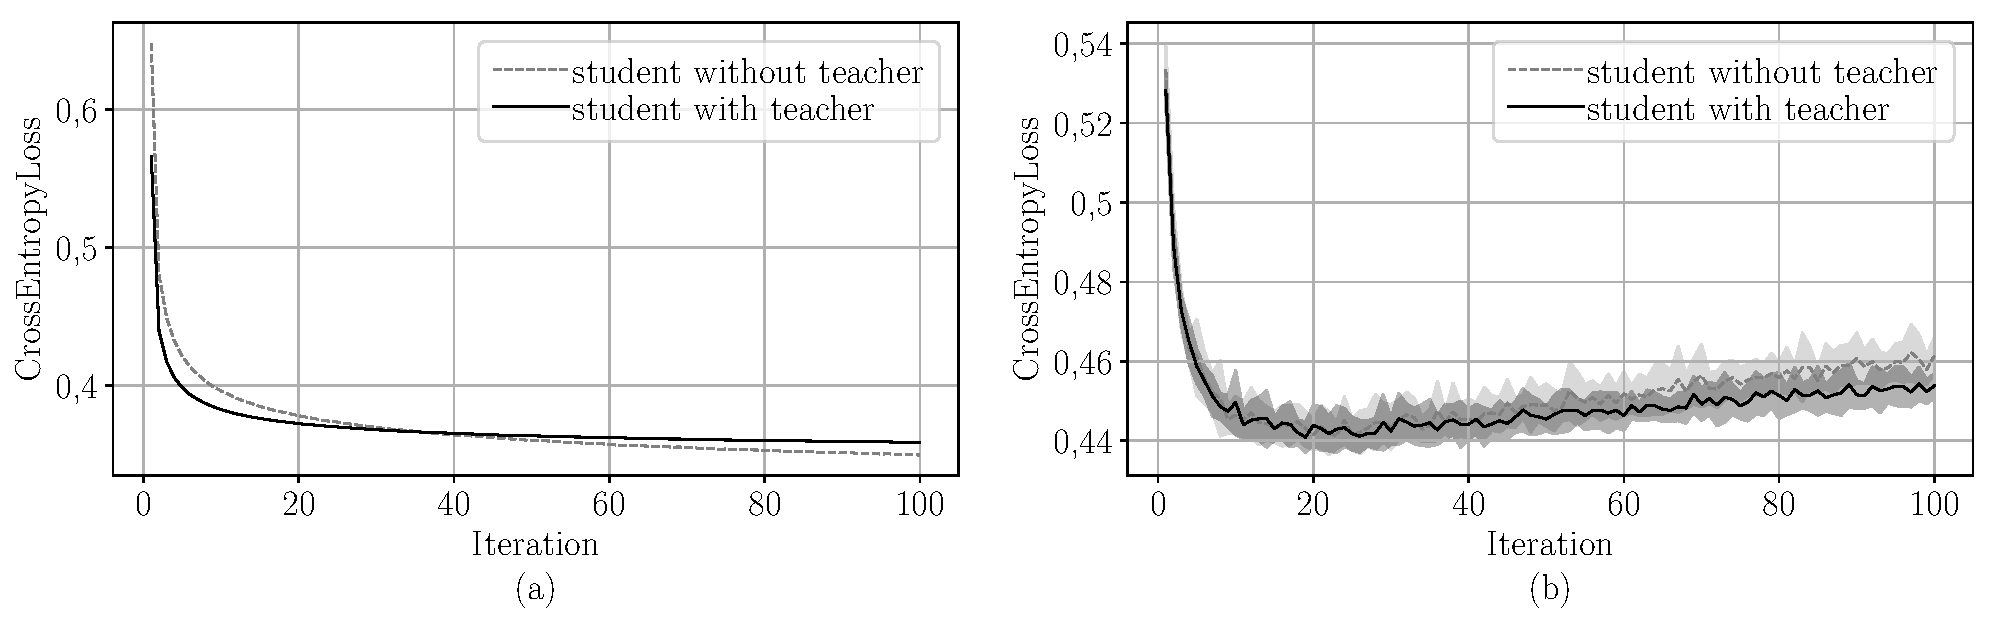
\includegraphics[width=1\textwidth]{figures/mnist_loss}
}

Кросс-энтропийная функция ошибки модели ученика: a) на обучающей выборке; b) на тестовой выборке.

На графике видно, что обе модели начинают переобучатся после 30-й итерации, но модель, которая получена путем дистилляции переобувается не так быстро, что следует из того, что ошибка на тестовой выборке растет медленней, а на обучающей выборке падает также медленней.



\end{frame}
%----------------------------------------------------------------------------------------------------------

\begin{frame}{Синтетический эксперимент: распределение классов}
\justifying
{\center
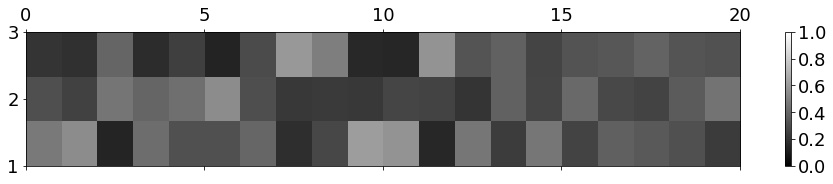
\includegraphics[width=0.7\textwidth]{figures/syn_real_distr}\\
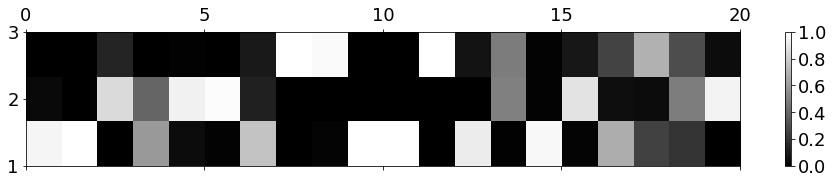
\includegraphics[width=0.7\textwidth]{figures/syn_without_teacher_distr}\\
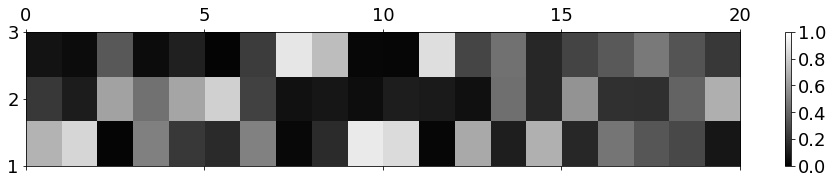
\includegraphics[width=0.7\textwidth]{figures/syn_with_teacher_distr}\\
}
Столбец --- вероятность класса, строка --- объекты.
Сверху вниз: истинное распределение; без учителя; с учителем.

Модели ученика, которая использует информацию учителя более точно восстанавливает вероятности классов в пространстве оценок чем модель ученика, которая не использует информации учителя.
\end{frame}
%----------------------------------------------------------------------------------------------------------

\begin{frame}{Синтетический эксперимент: анализ параметра $\lambda$ и $T$}
\justifying
\begin{center}
{\center
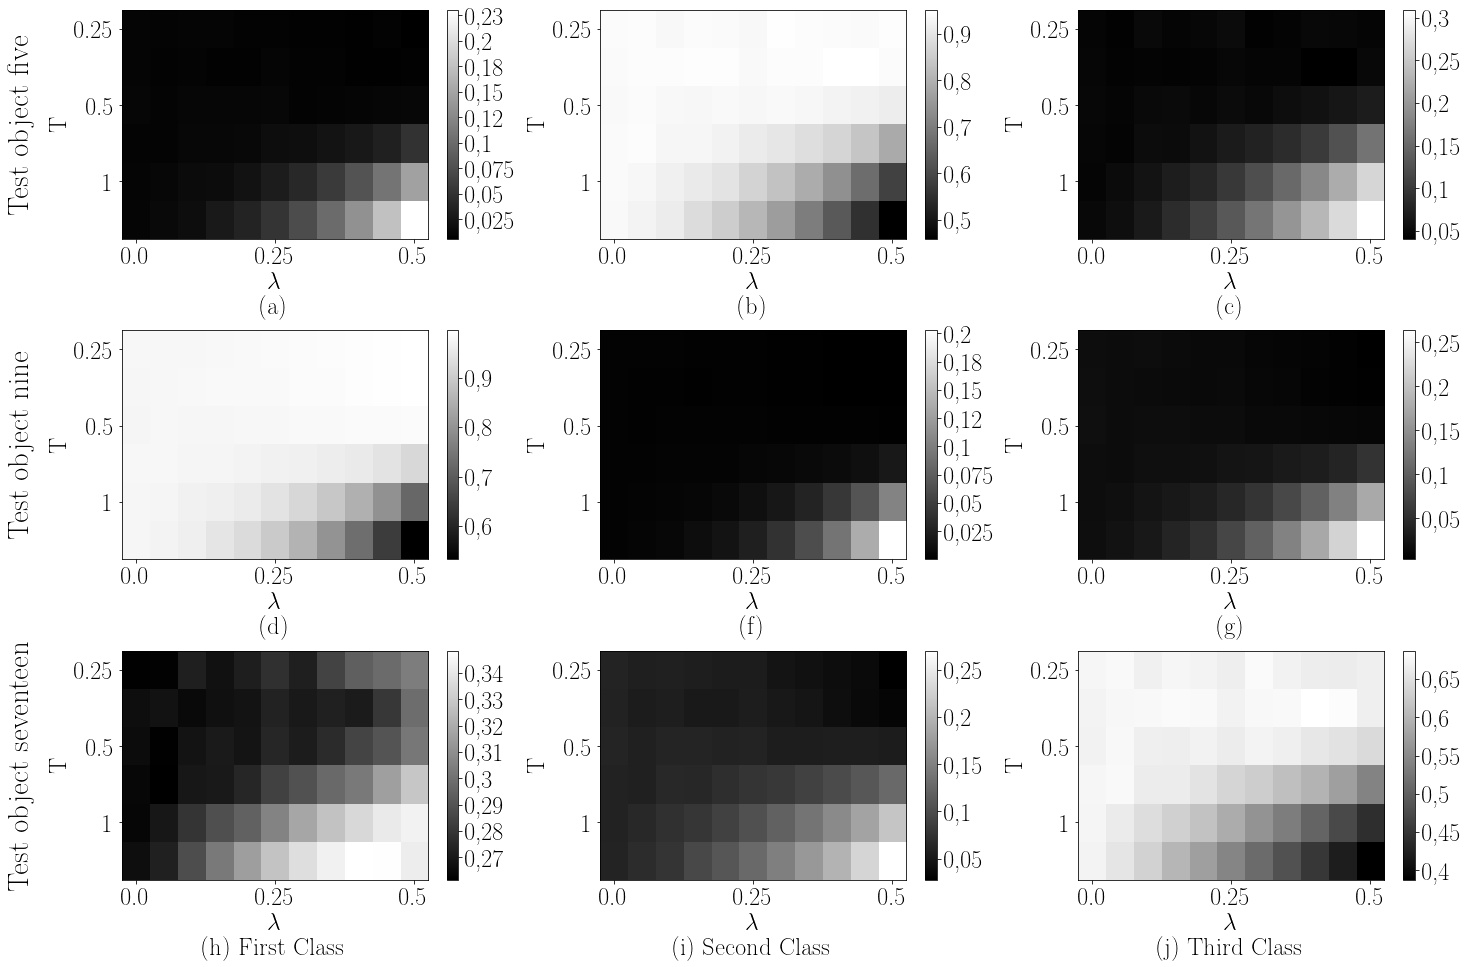
\includegraphics[width=0.8\textwidth]{figures/syn_T_lambda}
}
\end{center}

Зависимость распределения по классам при разных параметрах $\lambda$ и $T$.  Видно, что при увеличении температуры~$T$ распределение на классах становится более равномерным.

\end{frame}
%----------------------------------------------------------------------------------------------------------


\begin{frame}{Выборка Twitter Sentiment Analysis}
\justifying
В твитах была выполнена следующая предобработка:
\begin{itemize}
	\item все твиты были переведены в нижний регистр;
	\item все никнеймы вида~``@andrey'' были заменены на токен ``name'';
	\item все цифры были заменены на токен ``number''.
\end{itemize}

~\\
Описание моделей:
\begin{itemize}
	\item модель учителя: модель на основе Bi-LSTM с $\approx 30$ миллионов настраиваемых параметров;
	\item модель ученика: модель на основе предобученной модели BERT с $1538$ настраиваемых параметров.
\end{itemize}

\begin{table}[]
\begin{center}
\resizebox{\textwidth}{!}{
	\begin{tabular}{|l|c|c|c|}
	\hline
	\multicolumn{1}{|c|}{Model} & CrossEntropyLoss      & Accuracy             & StudentSize \\ \hline
	без учителя                 & $0{,}501 \pm 0{,}006$ & $0{,}747\pm 0{,}005$ & $1538$      \\ \hline
	с учителем                  & $0{,}489 \pm 0{,}003$ & $0{,}764\pm 0{,}004$ & $1538$      \\ \hline
	\end{tabular}
}
\end{center}
\end{table}
С таблицы видно, что при использовании учителя качество модели ученика увеличивается на $2\%$ по сравнению с аналогичной моделью без использования меток учителя.
\end{frame}
%----------------------------------------------------------------------------------------------------------


\begin{frame}{Сводная таблица вычислительного эксперимента}
\justifying

\begin{table}[]
\begin{center}
\resizebox{\textwidth}{!}{
	\begin{tabular}{|l|l|c|c|c|}
	\hline
	\multicolumn{1}{|c|}{Dataset} & \multicolumn{1}{c|}{Model} & CrossEntropyLoss      & Accuracy    &   StudentSize   \\ \hline
\hline
	
	\multirow{2}{*}{FashionMnist} & without teacher    &  $0{,}461 \pm 0{,}005$ & $0{,}841\pm 0{,}002$ & 7850 \\ \cline{2-5} 
                              & with teacher       & $0{,}453 \pm 0{,}003$ & $0{,}842 \pm 0{,}002$ & 7850\\ \hline
\hline
	\multirow{2}{*}{Synthetic}    & without teacher    & $0{,}225 \pm 0{,}002$ & $0{,}831\pm 0{,}002$ & 33 \\ \cline{2-5} 
                              &  with teacher       & $0{,}452 \pm 0{,}001$   & $0{,}828\pm 0{,}001$ & 33 \\ \hline
\hline
	\multirow{2}{*}{Twitter }    & without teacher    & $0{,}501 \pm 0{,}006$ & $0{,}747\pm 0{,}005$ & $1538$  \\ \cline{2-5} 
                              &with teacher       & $0{,}489 \pm 0{,}003$   & $0{,}764\pm 0{,}004$ & $1538$ \\ \hline
	\end{tabular}
}
\end{center}
\end{table}

В таблице показаны результаты вычислительного эксперимента для разных выборок. Из таблицы видно, что точность аппроксимации выборки учеником улучшается при использовании модели учителя при обучении.

\end{frame}
%----------------------------------------------------------------------------------------------------------

\begin{frame}{Заключение}
\justifying
Сделано:
	\begin{enumerate}
	\justifying
		\item поставлена вероятностная задача дистилляции моделей глубокого обучения;
		\item проведен теоретический анализ предложенной вероятностной задачи;
		\item результат анализа сформулирован в виде теорем: для задачи классификации, а также для задачи линейной регрессии;
		\item теорема для задачи линейной регрессии показала, что обучения модели линейной регрессии с учителем сводится к задаче линейной регрессии со скорректированными ответами;
		\item проведен вычислительный эксперимент для анализа предложенной модели.
	\end{enumerate}

Планируется:
	\begin{enumerate}
	\justifying
		\item обобщить предложенный метод на случай задачи регрессии более корректно;
		\item использовать байесовский подход выбора моделей машинного обучения для решения данной задачи.
	\end{enumerate}	

\end{frame}
%----------------------------------------------------------------------------------------------------------

\begin{frame}{Публикации по теме}
\justifying
\begin{enumerate}
\item \textit{Грабовой А.В., Бахтеев О.Ю., Стрижов В.В.} Определение релевантности параметров нейросети // Информатика и ее применения, 2019, 13(2).
\item \textit{Грабовой А.В., Бахтеев О. Ю., Стрижов В.В.} Введение отношения порядка на множестве параметров аппроксимирующих моделей // Информатика и ее применения, 2020, 14(2).
\item \textit{A. Grabovoy, V. Strijov.} Quasi-periodic time series clustering for human. Lobachevskii Journal of Mathematics, 2020, 41(3).
\item \textit{Грабовой А.В., Стрижов В.В.} Анализ выбора априорного распределения для смеси экспертов // Журнал Вычислительной математики и математической физики, 2021. 61(5).
\item \textit{Грабовой А.В., Стрижов В.В.} Анализ моделей привилегированного обучения и дистилляции // Автоматика и телемеханика, 2021 (текущая работа, на рецензировании).
\end{enumerate}

\end{frame}
%----------------------------------------------------------------------------------------------------------

\end{document} 